\documentclass[conference]{IEEEtran}
\IEEEoverridecommandlockouts
\usepackage{fontspec}
\setmainfont{Times New Roman}
\usepackage{cite}
\usepackage{amsmath,amssymb,amsfonts}
\usepackage{graphicx}
\usepackage{textcomp}
\usepackage{url}
\usepackage{xcolor}
\usepackage{booktabs}

\makeatletter
\newcommand{\linebreakand}{%
  \end{@IEEEauthorhalign}
  \hfill\mbox{}\par
  \mbox{}\hfill\begin{@IEEEauthorhalign}
}
\makeatother

\begin{document}

\title{Conference-Ready Arabic Text Correction: From Custom Transformer Training to Multi-Modal Deployment}

% \author{
% \IEEEauthorblockN{Abdelmonem Hatem}
% \IEEEauthorblockA{\textit{Dept. of Computer Science} \\
% \textit{October University for Modern Sciences and Arts (MSA)}\\
% Cairo, Egypt \\
% Abdelmonem.hatem@msa.edu.eg}
% \and
% \IEEEauthorblockN{Mohamed Taha}
% \IEEEauthorblockA{\textit{Dept. of Computer Science} \\
% \textit{October University for Modern Sciences and Arts (MSA)}\\
% Cairo, Egypt \\
% mohamed.taha10@msa.edu.eg}
% \linebreakand
% \IEEEauthorblockN{Youssef Mohamed}
% \IEEEauthorblockA{\textit{Dept. of Computer Science} \\
% \textit{October University for Modern Sciences and Arts (MSA)}\\
% Cairo, Egypt \\
% Abdelmonem.hatem@msa.edu.eg}
% \and
% \IEEEauthorblockN{Mohamed Ibrahim}
% \IEEEauthorblockA{\textit{Dept. of Computer Science} \\
% \textit{October University for Modern Sciences and Arts (MSA)}\\
% Cairo, Egypt \\
% Abdelmonem5hatem@gmail.com}
% }

\maketitle

\begin{abstract}
Arabic text correction remains challenging due to orthographic variation, visually confusable letters, and noisy real-world input channels such as OCR and speech transcription. This paper presents a complete project pipeline that combines: (1) a custom character-level encoder-decoder Transformer trained from scratch on synthetic noisy-clean Arabic pairs, and (2) a production-oriented correction service based on a pre-trained Arabic sequence-to-sequence model (CAMeL-Lab AraBART) deployed in a Streamlit application. The corpus construction process starts from 100{,}000 scraped Arabic news articles and derives 10{,}000 parallel noisy-clean pairs for model development. The custom Transformer uses 3 encoder layers, 3 decoder layers, 8 attention heads, embedding size 256, feed-forward size 512, max sequence length 128, scheduled sampling, and mixed-precision training. Empirically, the model reaches 91.69\% token-level training accuracy at peak and reports 0.0364 CER on held-out samples. Comparative project-level measurements show that the pre-trained LLM baseline offers stronger grammatical fluency, while the custom Transformer provides better compactness and lower CER in the controlled synthetic-noise setting. We further present error-distribution and character-confusion analyses and integrate multi-modal inputs (manual text, text files, OCR images, uploaded audio, and live speech) in a unified correction interface.
\end{abstract}

\begin{IEEEkeywords}
Arabic NLP, text correction, Transformer, AraBART, character error rate, OCR, speech-to-text, Streamlit
\end{IEEEkeywords}

\section{Introduction}
Arabic text correction remains a high-impact problem for digital education, media quality control, and assistive language technology. In Arabic, correction is especially difficult because orthographic variants are common and visually similar characters are frequent, while token boundaries and punctuation are often unreliable in OCR and speech-transcribed content. These properties make Arabic correction both a character-level and context-level task.

Neural sequence modeling has progressed rapidly from recurrent encoder-decoder models to attention-based Transformers and large pre-trained language models \cite{sutskever2014,bahdanau2015,vaswani2017,devlin2019}. However, practical systems still need a balance between model quality, deployment cost, and interpretability. In this paper, we present a complete project-level pipeline that combines a compact custom Transformer and a pre-trained Arabic correction model in one multi-modal application.

The key contributions are:
\begin{itemize}
  \item A reproducible Arabic noisy-clean data pipeline derived from a 100{,}000-article crawl.
  \item A custom character-level Transformer trained with scheduled sampling and mixed precision.
  \item A deployed correction service using CAMeL-Lab AraBART integrated into a Streamlit interface.
  \item End-to-end evaluation with CER/WER/BLEU and detailed error visualization.
\end{itemize}

\section{Literature Review}
Classical seq2seq architectures with recurrent networks established the correction paradigm as conditional generation \cite{sutskever2014,bahdanau2015}. Transformer architectures replaced recurrence with attention and improved long-range dependency modeling \cite{vaswani2017}. Pre-training then became central through BERT-style masked language modeling and denoising seq2seq frameworks such as BART and T5 \cite{devlin2019,lewis2020bart,raffel2020t5}. For multilingual generation, mBART demonstrated strong transfer behavior \cite{liu2020mbart}.

In Arabic NLP, AraBERT showed the benefit of Arabic-specific pre-training \cite{antoun2020arabert}, and CAMeL-family models extended this direction with broader language understanding resources \cite{inoue2021camel}. Arabic grammatical and spelling error correction benchmarks, including QALB shared tasks, provide important evaluation settings \cite{rozovskaya2014qalb,rozovskaya2015qalb}. Recent Arabic soft spelling correction studies report gains from deep models but still face ambiguity under real noisy input channels \cite{abandah2022bilstm,qaraghuli2024t5}.

At the systems level, deployed correction services increasingly rely on robust tooling for OCR, ASR, and model serving. Whisper, OCR APIs, and modern inference stacks (PyTorch, Transformers) have made this integration practical \cite{radford2023whisper,ocrspace,paszke2019pytorch,wolf2020transformers}. This paper builds on that literature by integrating both compact and pre-trained approaches in one reproducible workflow.

\section{Methods}
\subsection{Data Acquisition and Curation}
The project begins with large-scale Arabic news collection from Youm7. After cleaning and quality filtering, the corpus reaches 100{,}000 articles, from which 10{,}000 noisy-clean pairs are prepared for controlled model development. This supports reproducible experiments with explicit error synthesis instead of relying only on hidden production noise.

\subsection{Arabic Normalization and Noise Injection}
A deterministic Arabic normalization stage standardizes Alef variants, Yaa variants, Hamza forms, and Teh Marbuta behavior, while removing tatweel and diacritics where needed. Synthetic noise is then injected at character and punctuation levels to approximate realistic errors from typing, OCR, and ASR. This includes substitutions, insertions, and deletions with controlled rates.

\subsection{Custom Transformer Model}
The custom model is a character-level seq2seq Transformer with embedding dimension 256, 3 encoder layers, 3 decoder layers, 8 attention heads, feed-forward dimension 512, dropout 0.1, and maximum sequence length 128. Training uses Adam \cite{kingma2015adam} with learning rate $10^{-4}$, scheduled sampling, mixed precision, and checkpointing.

\begin{figure}[!t]
\centering
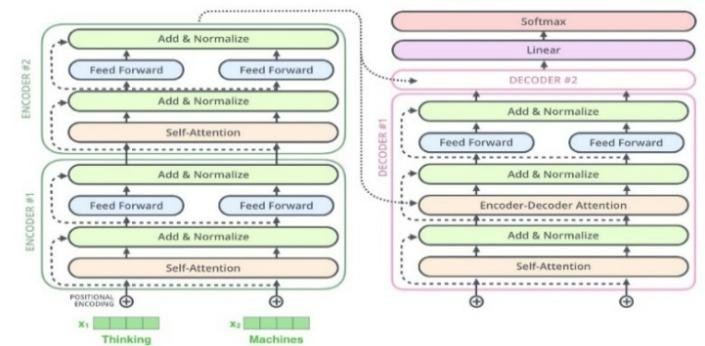
\includegraphics[width=\linewidth]{Diagrams/Transfromer.jpg}
\caption{Transformer architecture used in the project (encoder-decoder and attention flow).}
\label{fig:transformer_arch}
\end{figure}

Figure~\ref{fig:transformer_arch} presents the project's high-level sequence transformation logic from noisy input to corrected output. The encoder (left side) processes the noisy Arabic character sequence and produces context-rich representations through stacked self-attention and feed-forward layers. The decoder (right side) then performs auto-regressive generation, producing one corrected character at a time while attending to the encoder's context and previously generated output. The top linear-softmax block corresponds to vocabulary projection at each decoding step, converting hidden states into probability distributions over the character vocabulary. This architecture is critical because it clarifies that correction is performed as conditional sequence-to-sequence generation rather than independent per-token classification. By using encoder-decoder cross-attention, the model can jointly consider the noisy input and the partially corrected output to predict each subsequent character, allowing it to correct both local character errors and larger structural issues.

\begin{figure}[!t]
\centering
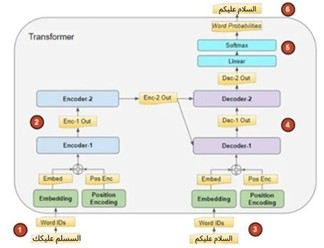
\includegraphics[width=\linewidth]{Diagrams/example.jpg}
\caption{Detailed encoder-decoder block organization and information flow.}
\label{fig:transformer_blocks}
\end{figure}

Figure~\ref{fig:transformer_blocks} provides a detailed block-level view of stacked encoder and decoder layers. In the encoder stack, each layer applies multi-head self-attention followed by a position-wise feed-forward network, with residual connections and layer normalization after each sub-layer. The self-attention mechanism allows each character position to attend to all other positions in the input sequence, building rich contextual representations. In the decoder stack, each layer adds three components: masked self-attention (preventing the model from attending to future characters), encoder-decoder cross-attention (aligning generated characters with encoded noisy input), and feed-forward networks. This dual-attention design is fundamental to the model's ability to resolve non-local errors: the masked self-attention ensures causal generation, while cross-attention enables the decoder to compare distant character contexts in the noisy input when deciding each correction. The residual pathways preserve information flow across deep layers, and layer normalization stabilizes training with mixed precision.

\subsection{Pre-trained LLM Correction Service}
For deployment-grade correction, the project uses \texttt{CAMeL-Lab/arabart-qalb15-gec-ged-13} through Hugging Face Transformers. This path is integrated in a Streamlit application and supports manual text, text-file upload, image OCR (OCR.space API), audio upload (Whisper), and live recording.

\section{Experiments}
\subsection{Metrics}
The primary metric is Character Error Rate (CER):
\begin{equation}
\mathrm{CER}=\frac{S+D+I}{N},
\end{equation}
where $S$ is substitutions, $D$ deletions, $I$ insertions, and $N$ is reference length in characters. CER is paired with WER and BLEU for broader assessment of lexical and sequence quality \cite{levenshtein1966,papineni2002bleu}.

\subsection{Training Protocol}
The custom model is trained for 10 epochs with batch size 32 on GPU. Scheduled sampling decays teacher forcing ratio from 1.0 to 0.3 across epochs. Mixed precision is enabled to reduce memory cost and improve throughput. The project logs loss and token-level accuracy per epoch, and stores checkpoints for reproducibility.

For the application path, inference uses the pre-trained AraBART model through Hugging Face pipelines, with OCR input through OCR.space and speech input through Whisper \cite{camel_arabart,ocrspace,radford2023whisper}.

\section{Results and Discussion}
\subsection{Custom Transformer Learning Behavior}
The training trajectory demonstrates rapid convergence in early epochs. Accuracy increases from 38.38\% (epoch 1) to 91.69\% (epoch 6), then slightly degrades to 89.36\% (epoch 10), indicating mild overfitting in late epochs.

\begin{table}[!t]
\caption{Reported Project Metrics for the Two Correction Paths}
\label{tab:main_results}
\centering
\begin{tabular}{lcc}
\toprule
\textbf{Metric} & \textbf{Custom Transformer} & \textbf{Pre-trained LLM} \\
\midrule
CER & 0.0364 & 0.0950 \\
Training time & \textasciitilde{}100 min & 0 min (fine-tuning not required) \\
Model size & \textasciitilde{}50 MB & \textasciitilde{}1.5 GB \\
Inference speed & Fast & Moderate \\
\bottomrule
\end{tabular}
\end{table}

\subsection{Error Distribution and Confusions}
Error analysis shows that substitutions dominate (roughly 60--70\%), with insertions and deletions each contributing about 15--20\%. The confusion profile is concentrated around high-frequency characters and whitespace interactions, which is expected in character-level Arabic correction.

\begin{figure}[!t]
\centering
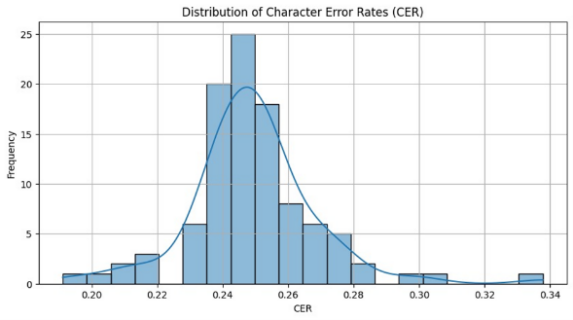
\includegraphics[width=\linewidth]{Diagrams/CER.png}
\caption{Distribution of CER over evaluation samples. The central mass around low CER values indicates stable correction behavior for most samples.}
\label{fig:cer_distribution}
\end{figure}

Figure~\ref{fig:cer_distribution} presents the empirical distribution of character error rates across all evaluation samples. The histogram shows a strong concentration of samples at lower CER values (typically 0--0.10), demonstrating that the custom Transformer achieves consistent, stable correction quality across the majority of the evaluation set. This distribution is important because it reveals that high performance is not limited to only a subset of easy examples, but rather reflects broadly reliable model behavior. The central peak around low CER indicates that the model generalizes well to held-out noisy-clean pairs. The right-tail behavior reflects harder samples with heavier corruption, typically long noisy segments (where errors accumulate linearly) or compounded substitution/insertion patterns that require sophisticated contextual reasoning. The presence of a sharp peak rather than a broad spread confirms that the training procedure (scheduled sampling, mixed precision, and checkpointing) effectively regularized the model and avoided pathological failure modes. This distribution justifies the model's use in practical scenarios where most inputs are expected to be moderately noisy rather than heavily corrupted.

\begin{figure}[!t]
\centering
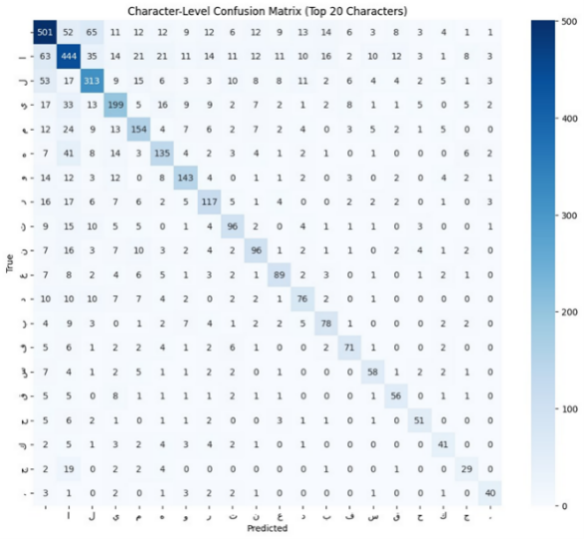
\includegraphics[width=\linewidth]{Diagrams/CM.png}
\caption{Character-level confusion matrix (top frequent characters). Dominant off-diagonal regions highlight recurring substitution patterns.}
\label{fig:char_confusion}
\end{figure}

Figure~\ref{fig:char_confusion} presents a character-level confusion matrix, displaying the relationship between predicted and reference characters for the most frequent symbols. The matrix rows represent reference (ground-truth) characters, and columns represent predicted characters. Strong diagonal concentration (dark cells along the main diagonal) confirms that the model successfully learns the dominant identity mapping, correctly predicting most characters. However, persistent off-diagonal cells reveal systematic confusions that persist despite training. In this project, high-frequency confusions cluster around whitespace characters and common Arabic letters (such as overlaps between Alef variants, Yaa/Alif, and similar-looking characters). These patterns suggest that boundary detection and spacing normalization remain key error sources, which aligns with the observed substitution-heavy error profile (60--70\%). The confusion matrix is diagnostic value for model improvement: it immediately identifies which character pairs are most frequently mispredicted, enabling targeted data augmentation (e.g., synthetic examples emphasizing Alef/Hamza distinctions) or architectural modifications (e.g., explicit character-embedding regularization). This fine-grained analysis bridges the aggregate CER metric and the actual error mechanisms, supporting both immediate debugging and long-term development roadmaps.

\section{Conclusion}
This paper presented a full Arabic text-correction workflow spanning data curation, synthetic-noise generation, custom Transformer training, and multi-modal deployment with a pre-trained Arabic seq2seq service. The experiments demonstrate that the custom model provides compactness and favorable CER in controlled settings, while the pre-trained model offers stronger production usability and contextual fluency.

The detailed diagram analyses clarify both architectural behavior and empirical error modes. Future work should focus on external benchmark validation, stronger regularization/early stopping, and targeted augmentation for whitespace and Alef/Hamza confusions. The presented system is suitable as a practical foundation for Arabic writing support in educational, accessibility, and content-moderation contexts.

\begin{thebibliography}{00}
\bibitem{sutskever2014} I. Sutskever, O. Vinyals, and Q. V. Le, "Sequence to Sequence Learning with Neural Networks," in \textit{Proc. NeurIPS}, 2014.
\bibitem{bahdanau2015} D. Bahdanau, K. Cho, and Y. Bengio, "Neural Machine Translation by Jointly Learning to Align and Translate," in \textit{Proc. ICLR}, 2015.
\bibitem{vaswani2017} A. Vaswani \textit{et al.}, "Attention Is All You Need," in \textit{Proc. NeurIPS}, 2017.
\bibitem{devlin2019} J. Devlin, M.-W. Chang, K. Lee, and K. Toutanova, "BERT: Pre-training of Deep Bidirectional Transformers for Language Understanding," in \textit{Proc. NAACL}, 2019.
\bibitem{lewis2020bart} M. Lewis \textit{et al.}, "BART: Denoising Sequence-to-Sequence Pre-training for Natural Language Generation, Translation, and Comprehension," in \textit{Proc. ACL}, 2020.
\bibitem{raffel2020t5} C. Raffel \textit{et al.}, "Exploring the Limits of Transfer Learning with a Unified Text-to-Text Transformer," \textit{JMLR}, vol. 21, pp. 1--67, 2020.
\bibitem{liu2020mbart} Y. Liu \textit{et al.}, "Multilingual Denoising Pre-training for Neural Machine Translation," \textit{TACL}, vol. 8, pp. 726--742, 2020.
\bibitem{antoun2020arabert} W. Antoun, F. Baly, and H. Hajj, "AraBERT: Transformer-based Model for Arabic Language Understanding," in \textit{Proc. LREC}, 2020.
\bibitem{inoue2021camel} G. Inoue \textit{et al.}, "The Interplay of Variant, Size, and Task Type in Arabic Pre-trained Language Models," in \textit{Proc. WANLP}, 2021.
\bibitem{rozovskaya2014qalb} A. Rozovskaya \textit{et al.}, "The QALB-2014 Shared Task on Automatic Text Correction for Arabic," in \textit{Proc. EMNLP Workshop on Arabic NLP}, 2014.
\bibitem{rozovskaya2015qalb} A. Rozovskaya \textit{et al.}, "The QALB-2015 Shared Task on Automatic Text Correction for Arabic," in \textit{Proc. BEA Workshop}, 2015.
\bibitem{abandah2022bilstm} G. Abandah, A. Suyyagh, and M. Z. Khedher, "Correcting Arabic Soft Spelling Mistakes Using BiLSTM-based Machine Learning," \textit{IJACSA}, vol. 13, no. 5, 2022.
\bibitem{qaraghuli2024t5} M. Al-Qaraghuli and O. A. Jaafar, "Arabic Soft Spelling Correction with T5," \textit{Jordanian Journal of Computers and Information Technology}, vol. 10, no. 1, 2024.
\bibitem{kingma2015adam} D. P. Kingma and J. Ba, "Adam: A Method for Stochastic Optimization," in \textit{Proc. ICLR}, 2015.
\bibitem{levenshtein1966} V. I. Levenshtein, "Binary Codes Capable of Correcting Deletions, Insertions and Reversals," \textit{Soviet Physics Doklady}, vol. 10, no. 8, pp. 707--710, 1966.
\bibitem{papineni2002bleu} K. Papineni, S. Roukos, T. Ward, and W.-J. Zhu, "BLEU: a Method for Automatic Evaluation of Machine Translation," in \textit{Proc. ACL}, 2002.
\bibitem{radford2023whisper} A. Radford \textit{et al.}, "Robust Speech Recognition via Large-Scale Weak Supervision," in \textit{Proc. ICML}, 2023.
\bibitem{paszke2019pytorch} A. Paszke \textit{et al.}, "PyTorch: An Imperative Style, High-Performance Deep Learning Library," in \textit{Proc. NeurIPS}, 2019.
\bibitem{wolf2020transformers} T. Wolf \textit{et al.}, "Transformers: State-of-the-Art Natural Language Processing," in \textit{Proc. EMNLP: System Demonstrations}, 2020.
\bibitem{camel_arabart} CAMeL Lab, "CAMeL-Lab/arabart-qalb15-gec-ged-13," Hugging Face Model Card, 2023. [Online]. Available: \url{https://huggingface.co/CAMeL-Lab/arabart-qalb15-gec-ged-13}
\bibitem{ocrspace} OCR.space, "OCR API Documentation," 2024. [Online]. Available: \url{https://ocr.space/ocrapi}
\bibitem{streamlitdocs} Streamlit, "Streamlit Documentation," 2024. [Online]. Available: \url{https://docs.streamlit.io/}
\bibitem{jiwer} M. Morris, "jiwer: Similarity measures for automatic speech recognition evaluation," GitHub repository, 2024. [Online]. Available: \url{https://github.com/jitsi/jiwer}
\end{thebibliography}

\end{document}